\documentclass[xcolor={dvipsnames},pdf, hyperref={colorlinks=true, citecolor=ForestGreen, linkcolor=BlueViolet, urlcolor=Magenta}]{beamer}
\usetheme{Frankfurt}  
\usecolortheme{whale}
\usepackage{tikz} 
\usepackage{amsmath}
\usepackage{amsthm}
\usepackage{amssymb}              % used for \eqref{} in this document
\usepackage{dsfont}
\usepackage{hyperref}
\usepackage{threeparttable}
\usepackage{multirow}
\graphicspath{{Figures/}}
\usepackage{booktabs}
\usepackage{tikz}
\newtheorem{exmp}{Example}[section]
\usepackage{subcaption}
\usepackage{adjustbox}
\usepackage{graphicx}
\usepackage[mathscr]{euscript}
\usepackage{remreset}% tiny package containing just the \@removefromreset command
\makeatletter
\@removefromreset{subsection}{section}
\makeatother
\setcounter{subsection}{1}
\usepackage{float}
\usepackage{sgamevar}
\usepackage{sgame}

\newcommand{\defn}[1]{\textbf{#1}}


%Instructor version
\newcommand{\blank}[0]{}
\newcommand{\ddp}[1]{{\textcolor{ForestGreen}{#1}}} 
\newcommand{\dd}[1]{{\underline{\textcolor{ForestGreen}{#1}}}}

%Student version
%\newcommand{\blank}[0]{\vspace{2em}}
%\newcommand{\dd}[1]{\underline{\hspace{3cm}}} 
%\newcommand{\ddp}[1]{}

\addtobeamertemplate{navigation symbols}{}{%
	\usebeamerfont{footline}%
	\usebeamercolor[fg]{footline}%
	\hspace{1em}%
	\insertframenumber/\inserttotalframenumber
}

\section{Class Details}

%% preamble
\title{Principles of Economics}
\author{David A. D\'iaz}
\institute{UNC Chapel Hill}
\date{}

\AtBeginSection[] %Section links on slides

\begin{document} 
	
	\begin{frame}
		
		\titlepage
		
	\end{frame}
	
\begin{frame}{Table of Contents}
	
	\tableofcontents
\end{frame}


\begin{frame}{About Me (Less Fun)}
	\begin{itemize}
		\item 4$^{th}$ year Economics PhD student at UNC
		\item Appalachian State University alumnus
		\begin{itemize}
			\item Majors: Actuarial Science, Economics
			\item Minors: Statistics, Physics
		\end{itemize}
		\item Research interests: Migration, development, labor, demography
	\end{itemize}
\end{frame}


\begin{frame}{About Me (More Fun)}
	\begin{itemize}
		\item Fav. Music: T\O P, Arctic Monkeys, Glass Animals, alt-J, Two Door Cinema Club (allegedly ``angsty'')
		\begin{itemize}
			\item 2016 Top Song: Gooey (Glass Animals)
			\item 2017 Top Song: Local Long Distance Relationship (Saint Motel)
		\end{itemize}
		\item Fav. TV: It's Always Sunny, Archer, Wilfred, Arrested Development, 30 Rock, Real Housewives of Atlanta
		\item Fav. Movies: Fantastic Mr. Fox , Kiss Kiss Bang Bang, The Social Network, No Country for Old Men
	\end{itemize}
\end{frame}

\begin{frame}{About Me (More Fun)}
	\begin{itemize}
		\item Fav. Team: FC Barcelona
		\item Celebrity Crush: Kevin Spacey
		\item B\ae s: Elizabeth (main) \& Stella (side)
		\item Likes: Beer, t-shirts, normal shoes, Tina Fey
		\item Dislikes: Gyms, loud chewing, open-toed shoes, students packing up early $\sim$ shade emoji $\sim$
	\end{itemize}
\end{frame}

\begin{frame}{B\ae s}
	\begin{figure}
		\centering
		
\includegraphics[scale=.20]{bae2.pdf}
		\caption{Stella Artois D\'iaz }
	\end{figure}
\end{frame}



\begin{frame}{Administrative Details}
	
	\begin{itemize}
	\item \textbf{Email:} \url{diazda@live.unc.edu} 
	\item \textbf{Office:} Phillips Hall Annex 103A
	\item \textbf{Office Hours:} Tues/Friday 11:30am-1pm
	\item \textbf{Website:} \href{https://sakai.unc.edu/portal/site/2c4d5bc8-5222-46ac-bcad-18681c7e9ce9}{https://sakai.unc.edu}
				
	\end{itemize}
	
\end{frame}




	\begin{frame}{Textbook}
		\begin{itemize}
			\item N. Gregory Mankiw, \textit{Principles of Economics}, 8$^{th}$ edition
			\begin{itemize}
				\item Note: 7$^{th}$ or 6$^{th}$ edition probably work fine, but it is your responsibility to match up content.
				\item Any assigned readings from the text are fair game for exams unless told otherwise.
			\end{itemize}
	\end{itemize}
	\end{frame}


	\begin{frame}{Grade Components}
	\begin{itemize}
		\item Course grades are determined by the following:
		\begin{itemize}
			\item Participation: 10\%
			\item Homework: 25\%
			\item Exam 1: 	20\%
			\item Exam 2: 20\%
			\item	Final Exam: 25\% 
		\end{itemize}
		\item The grading scale is as follows:
		
		\begin{center}
			\begin{tabular}{ p{3.5cm} p{3.5cm} }
				A: 93 -- 100 &  C+: 77 -- 79.99\\
				A--: 90 -- 92.99 & C: 73 -- 76.99\\
				B+: 87 -- 89.99 & C--: 70 -- 72.99\\
				B: 83 -- 86.99 & D+: 65 -- 69.99\\
				B--: 80 -- 82.99 & D: 60 -- 64.99\\
				& F: $<$ 60
			\end{tabular}
		\end{center}
		
		\item Grades will be regularly updated on Sakai. Please bring up any discrepancies in a timely manner (within $\sim$1 week). 
	\end{itemize}
		

	\end{frame}
	
	\begin{frame}{Participation \& Problem Sets}
		\begin{itemize}
			\item Participation grade will be based on attendance, class demeanor, and effort level.
			\item Six problem sets with solutions are posted on Sakai.
			\begin{itemize}
				\item Intended to be study guides for exams.
				\item You are encouraged to work through these individually and with others.
			\end{itemize}
		\end{itemize}
	\end{frame}


	\begin{frame}{Homework}
	\begin{itemize}
			\item Six \textbf{graded} homeworks corresponding to each problem set will be given on Sakai during the semester.
		\begin{itemize}
			\item 20 questions from the relevant material
			\item 1 writing assignment per homework 
			\item Due at 11:55PM on the assigned date
			\item No late submissions (10 minute grace period)
			\item Open book/note/classmate.
			\item See syllabus for due dates (note: these are subject to change).
		\end{itemize}
	\end{itemize}
	\end{frame}
	

	
		\begin{frame}{Exams}
			
			\begin{itemize}
				\item Two in-class exams will take place during regular class hours. Each is worth 20\% of the final grade.
				\begin{itemize}
					\item Exam 1: May 30
					\item Exam 2: June 9
				\end{itemize}
				\item Our cumulative final exam is scheduled on June 21 from 8-11am.
				\item All exams will be closed book/note. You will be allowed the use of a \textbf{basic} calculator.
					 \begin{figure}
					 	\centering
					 	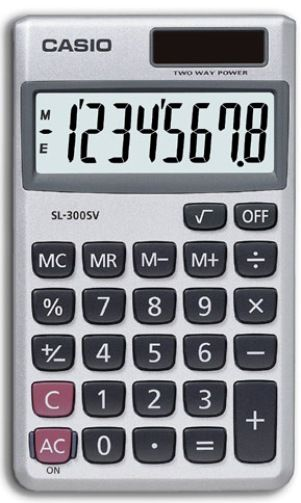
\includegraphics[width=.2\linewidth]{basic.jpg}
					 \end{figure}
			\end{itemize}
			
		\end{frame}
	
\begin{frame}{Policies \& Expectations}
	
		\begin{itemize}
			
			\item Regular attendance and participation is strongly encouraged. It is \textbf{your} responsibility to get any notes/announcements you may have missed from a classmate.
			\item Be respectful to both me and your classmates.
			\item Emails should be written in a professional manner.
				\begin{itemize}
					\item Use your UNC email, as email from other clients may end up in spam.
					\item I will do my best to respond to emails within 24 hours. If you have not heard back in 48 hours, please follow up to make sure your email was received.
				\end{itemize}  
		\end{itemize}

	
\end{frame}

\begin{frame}{Lectures}
\begin{itemize}
	\item Slides and the board will both be used to present material throughout the course.
		\begin{itemize}
			\item Data and concepts will mostly be presented on slides.
			\item Exposition, diagrams, and math will generally be done on the board.
		\end{itemize}
	\item Slides will generally be posted at least 24 hours before the corresponding class meeting.
\end{itemize}
\end{frame}

\begin{frame}{General Advice}
	
\begin{itemize}
	\item Bring a copy of the lecture slides to class.
	\item Keep up with the material! Work through each day's questions on the problem sets/homework as we go.
	\item Read the book \textbf{prior} to lecture. Reread the parts you are still unsure of afterwards.
	\item Try each problem set on your own at least once before working through it with others.
	\item Economics is best learned by working through problems. Practice, practice, practice!
\end{itemize}
		
\end{frame}


\begin{frame}{General Advice}
	
	\begin{itemize}
	\item Get in touch with me early if you are struggling with the material 
	\item The EconAid Center will also be available during the summer in Gardner 009
	\begin{itemize}
		\item Mondays and Fridays 1-3pm; Tuesday-Thursday 3-5pm (5/17-6/2)
		\item Monday-Friday 1-3pm (6/2-6/21)
	\end{itemize}
	\end{itemize}
	
\end{frame}

\section{Introduction to Economics}

\begin{frame}{What is Economics?}
	
\begin{itemize}
	\item The purpose of this course is to introduce you to a new way of looking at the world. 
	\item The course focuses on core economic concepts and introduces you to some basic models that economists use to make sense of what they observe around them. 
	\item We will also explore how economists analyze the impact of different policies within the context of these models and determine whether the policy will have the intended - or an unintended - outcome. 
	\item Throughout the course, I hope to increase your interest in economics and the role it can play in your everyday decision making.
\end{itemize}
	
\end{frame}

\begin{frame}{What is Economics?}
\begin{itemize}
	\item \defn{Economics is}
	\begin{enumerate}
		\item The study of how society manages its scarce resources.
		\item The study of decision making.
	\end{enumerate}

	\item \defn{Scarcity:} The limited nature of society's resources. Examples: Limited government revenue, land, income, time, etc.
	
	
\item	\defn{Microeconomics:} The study of economics that focuses on the individual parts of the economy (e.g., supply \& demand, firm behavior, etc.)

\item \defn{Macroeconomics:}  The study of economics that looks at the economy as a whole. (e.g., economic growth, inflation, etc.)
\end{itemize}
\end{frame}



\begin{frame}{What is Economics?}
	
	\begin{itemize}
		\item The Economic way of thinking
			\begin{itemize}
					\item involves analytical and objective thinking.
					\item makes use of the scientific method.
					\item uses \textit{abstract} models to help explain how the real world works.
			\end{itemize}
		\item Assumptions
			\begin{itemize}
				\item simplify the world and make it easier to understand.
				\item The ``art'' lies in deciding which assumptions to use. Different assumptions are used to answer different questions.
			\end{itemize}
		\item Sometimes these assumptions might seem unrealisitc. As you continue to study economics, assumptions are relaxed in order to create more realistic, albeit harder to solve, models.
	\end{itemize}
	
\end{frame}

\begin{frame}{Positive and Normative Analysis}
	\begin{itemize}
		\item \defn{Positive Analysis:} Analysis of how the world \underline{is}.
	
		\item \defn{Normative Analysis:} Analysis of how the world \underline{should be}.
	
		\item The key difference is in how their validity is judged.
		 \begin{itemize}
		 	\item Positive statements can be analyzed using data/facts, while normative statements involve value judgments.
		 \end{itemize}
	\end{itemize}
\end{frame}

\begin{frame}{Positive and Normative Analysis}
	\begin{exmp}
	Suppose you hear economists say each of the following statements. Are they positive or normative?
	\begin{enumerate}
		\item ``An increase in the minimum wage will cause a decrease in employment among the least-skilled.'' 
		\item ``We should lower taxes on the rich in order to stimulate the economy.'' 
		\item ``The income gains from increasing the minimum wage are worth more than any small decrease in employment.''
	\end{enumerate}
\end{exmp}
\ddp{\pause Positive; Normative; Normative}
\end{frame}



\begin{frame}{How People Make Decisions}
	\begin{itemize}
		\item \textbf{Principle 1: People Face Trade-offs}
			\begin{itemize}
					\item Come to class or sleep in.
					\item Go out on a Thursday night or do your homework.
					\item Societal tradeoff: Efficiency (biggest pie) vs. Equality (distribution of the pie).
			\end{itemize}
		\item 	\textbf{Principle 2: The Cost of Something is What You Give Up to Get It}

		\begin{itemize}
			\item \defn{Opportunity Cost:} The value of \underline{the next best alternative} you give up to obtain something.
			\item Note that this is not always in dollars \& cents. You could give up time or pure ``enjoyment.'' Time inherently has value, but ``enjoyment'' is harder to quantity. 
		\end{itemize}

		
		\begin{exmp}
			What is the opportunity cost of coming to class? 
		\end{exmp} 
		\pause \ddp{The value of the next best alternative. Sleeping in, time studying, etc.}
	\end{itemize}
\end{frame}



\begin{frame}{How People Make Decisions}
	\begin{exmp} 
		Suppose you currently pay \$10,000 a year for tuition, \$500 for books, and \$6,000 for room and board. If you quit school now, you could get a job paying \$25,000 a year and your costs of living would be identical to your room and board currently. What is your opportunity cost of going to college?
	\end{exmp}
		\ddp{\pause What are you giving up? \\
			1. Actual costs of college (tuition, books, room \& board) \\
			2. Salary you could be earning, minus room \& board
		\[OC = (10K + 500 + 6K) + (25K - 6K) = \$35,500\]}
\end{frame}

\begin{frame}{How People Make Decisions}
	\begin{exmp} 
		Who has a higher opportunity cost of going to college?
		\begin{enumerate}[(a)]
			{\setlength\itemindent{25pt}\item A famous actor who wishes to return to college to finish his degree.}
			{\setlength\itemindent{25pt}\item A young math whiz who will earn a high salary after the completion of her degree.}
		\end{enumerate}
	\end{exmp}
		\pause \ddp{The famous actor is giving up a high salary to return to school, while the math whiz is only giving up the wages she would earn without her degree which are much lower.}
\end{frame}

\begin{frame}{How People Make Decisions}
	\begin{itemize}
		\item \textbf{Principle 3: Rational People Think at the Margin}
		\item \defn{Rational Person:} A person who systemically and purposefully does the best they can to achieve their objective.
		
		\item \defn{Marginal Benefit:} The extra benefit from consuming one more unit of an item.
		
		\item \defn{Marginal Cost:} The additional cost from consuming one more unit of an item.
		
		\item \defn{Sunk Cost:} A cost that has already been incurred and cannot be recovered. These should be ignored when making a decision (``water under the bridge,'' ``don't cry over spilled milk'').
	\end{itemize}
\end{frame}

\begin{frame}{How People Make Decisions}
\begin{exmp}
	You are enjoying a show at a local establishment and have had a few of your favorite drink. You paid a \$10 cover charge to get in. What should you consider when deciding if you will have another drink?
\end{exmp}
\pause \ddp{Sunk cost: cover charge already paid.\\
	Marginal benefit: Enjoyment/happiness from your drink.\\ 
	Marginal costs: Actual cost of the drink, any negative side effects
	\\ As long as $MB \ge MC$, drink up.}
\end{frame}

\begin{frame}{How People Make Decisions}
\begin{exmp}
	\scriptsize
David is trying to figure out how many beers he should buy after grading his Econ 111 final exams. Table \ref{tab5} shows his marginal benefit for each additional beer as well as the total cost of each beer which includes the price of the beer along with the dollar cost of headache medicine, lost time, etc. each beer would have. 
\begin{table}[H]
	\caption{WTP and Costs of Beer}
	\label{tab5}
	\centering
	\begin{tabular}{ c|c|c} 
		
		Beer & MB & Total Cost \\
		\hline
		1st & \$6.00 & \$4.50  \\
		2nd & \$6.00 & \$9.50 \\
		3rd & \$5.50 & \$15.00 \\
		4th & \$5.25 & \$21.00\\
		5th & \$5.00 & \$27.50  \\
		6th & \$4.50 & \$34.50 \\
	\end{tabular}
\end{table}	
Given this information, how many beers should he buy?	
\end{exmp}
\pause \ddp{Optimal amount is where $MB = MC =\$5.50$ at $Q=3$.}
\end{frame}

\begin{frame}{How People Make Decisions}
\begin{exmp} 
	Chip recently bought a fixer upper in Cancun. He paid \$145,000 with the intent of spending \$25,000 in repairs on order to resell it for \$200,000. Before he could start repairs, travel restrictions to Cuba were lifted, driving home prices in Cancun down. As a result, Chip has two options: (a) repair the house for \$25,000 and sell it for \$140,000, or (b) forgo the repairs and sell the house as is for \$120,000. Which option should Chip choose?
\end{exmp}
\pause \ddp{Sunk cost: \$145K. 
	\\ Option A: \$140K - 25K = \$115 gain.
	\\ Option B: \$120K gain. 
	\\ Chip should choose Choose option B.}
\end{frame}

\begin{frame}{How People Make Decisions}
	\begin{itemize}
	
	\item	\textbf{Principle 4: People Respond to Incentives}
	
		
	\item	\defn{Incentive:} Something that induces a person to act.
	
	\end{itemize}	
		
		\begin{exmp}
		\begin{itemize}
			\item How can I get you to show up to class? 
			\item Teacher incentives: how can we induce teachers to improve student test scores?
		\end{itemize}
		\end{exmp} 
		\pause \ddp{(i) Attendance grade, giving pop quizzes, etc.\\
		(ii) We can increase the opportunity cost of shirking by tying pay to student test scores, year-to-year progress, etc. Negative side effects: teaching to the test, cheating, etc.}
\end{frame}

\section{Production Possibilities Frontier}

\begin{frame}{The Production Possibilities Frontier}
\begin{itemize}
\item 	\defn{PPF:} A graph that shows the combinations of output that the economy can possibly produce given the available factors of production and the available production technology. 
	\begin{itemize}
		\item Factors of production: labor, capital, land
		\item Technology: Knowledge about the production process.
		\item Fairly simple two good model, but illustrates the first two principles of economics: trade-offs and opportunity costs.
	\end{itemize}
\end{itemize}
\end{frame}

\begin{frame}{The Production Possibilities Frontier}
	\begin{itemize}
	\item	Consider an economy that can produce either 1,000 tractors or 4,000 tubas if it devotes all of its resources to either good.
	\end{itemize}		
			\begin{figure}[H]
				\centering
				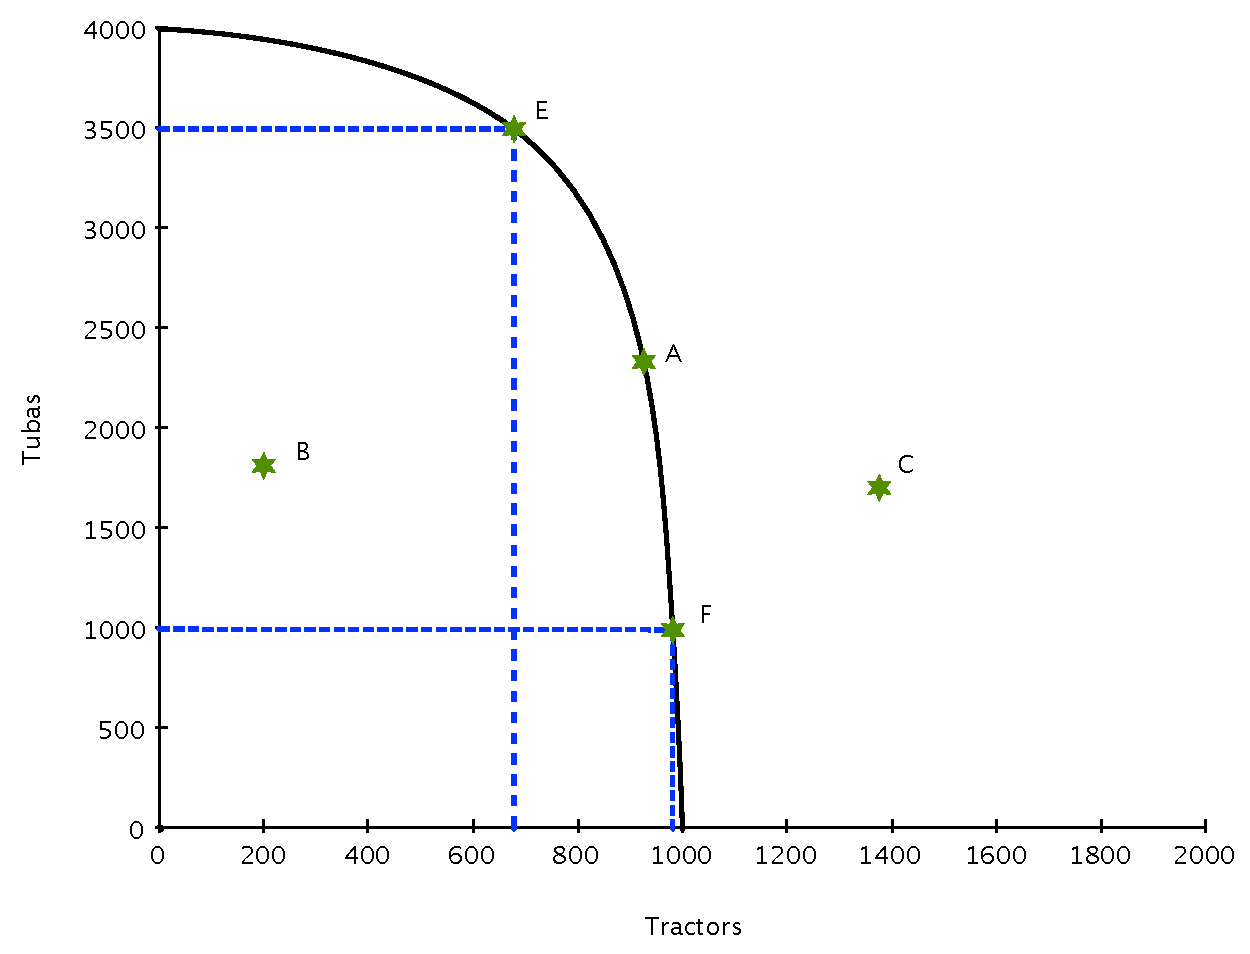
\includegraphics[scale=.3]{plot1.pdf}
				\caption{PPF for Tractors and Tubas}
				\label{ppf1}
			\end{figure}
\end{frame}


\begin{frame}{The Production Possibilities Frontier}
	\begin{itemize}
		\item 	Point \textbf{A} is said to be \dd{efficient}. 
		The economy is producing all it can given its resources.
		
		\item Point \textbf{B} is said to be \dd{inefficient}. 
		The economy is not producing all it can given its resources (e.g., underemployment of workers, available land not being utilized).
		
		\item Point \textbf{C} is said to be \dd{unfeasible}. The economy cannot support this output level with its current resources and technology.
	\end{itemize}
\end{frame}

\begin{frame}{The Production Possibilities Frontier}
\begin{itemize}
	\item	At point \textbf{E}, the economy is using most of its resources to produce tubas. 
	\begin{itemize}
		\item The resources best suited to producing tractors are being used in the tuba industry. 
		\item Thus, when we increase tractor production by one unit, we will only see a slight reduction in the number of tubas produced. 
	\end{itemize}
\end{itemize}	
\end{frame}

\begin{frame}{The Production Possibilities Frontier}
\begin{itemize}
		\item At point \textbf{F}, the resources best suited to producing tractors are already employed in that industry.
	\begin{itemize} 
		\item Producing an additional tractor means moving resources more suited to producing tubas out of the tuba industry and \item Thus there will be a large loss in the production of tubas.
	\end{itemize}
\end{itemize}
\end{frame}

\begin{frame}{The Production Possibilities Frontier}
	\begin{itemize}
	\item 	\textbf{\dd{Specialization of resources} leads to increasing opportunity costs along the PPF.}
	\item  	The slope of PPF is the OC of good on the \dd{x-axis}. 
	\item The reciprocal of the slope is the OC of good on the \dd{y-axis}.
	\end{itemize}
\end{frame}

\begin{frame}{The Production Possibilities Frontier}
	\begin{itemize}
		\item How do we move from point to point within a given PPF?
		  \begin{itemize}
		  	\item \ddp{Reemployment of existing resources.}
		  \end{itemize}
		\item How can we shift the entire PPF to produce at currently unfeasible points?
			\begin{itemize}
				\item \ddp{Changes in the factors of production.}  
				\item \ddp{Changes in technology.}
			\end{itemize}
	\end{itemize}
\end{frame}

\begin{frame}{The Production Possibilities Frontier}
		\begin{exmp} For each of the following, draw what would happen to the PPF.
			\begin{enumerate}
				\item The economy experienced a technological advance in the production of tractors.
				\item The country relaxed migration restrictions and saw an influx of more workers.
			\end{enumerate}
		\end{exmp} 
	\blank
	\blank
	\blank
	\blank
	
	
	\pause 
		
\begin{figure}[H]
	\centering
	\begin{subfigure}[t]{0.5\textwidth}
		\centering
		\ddp{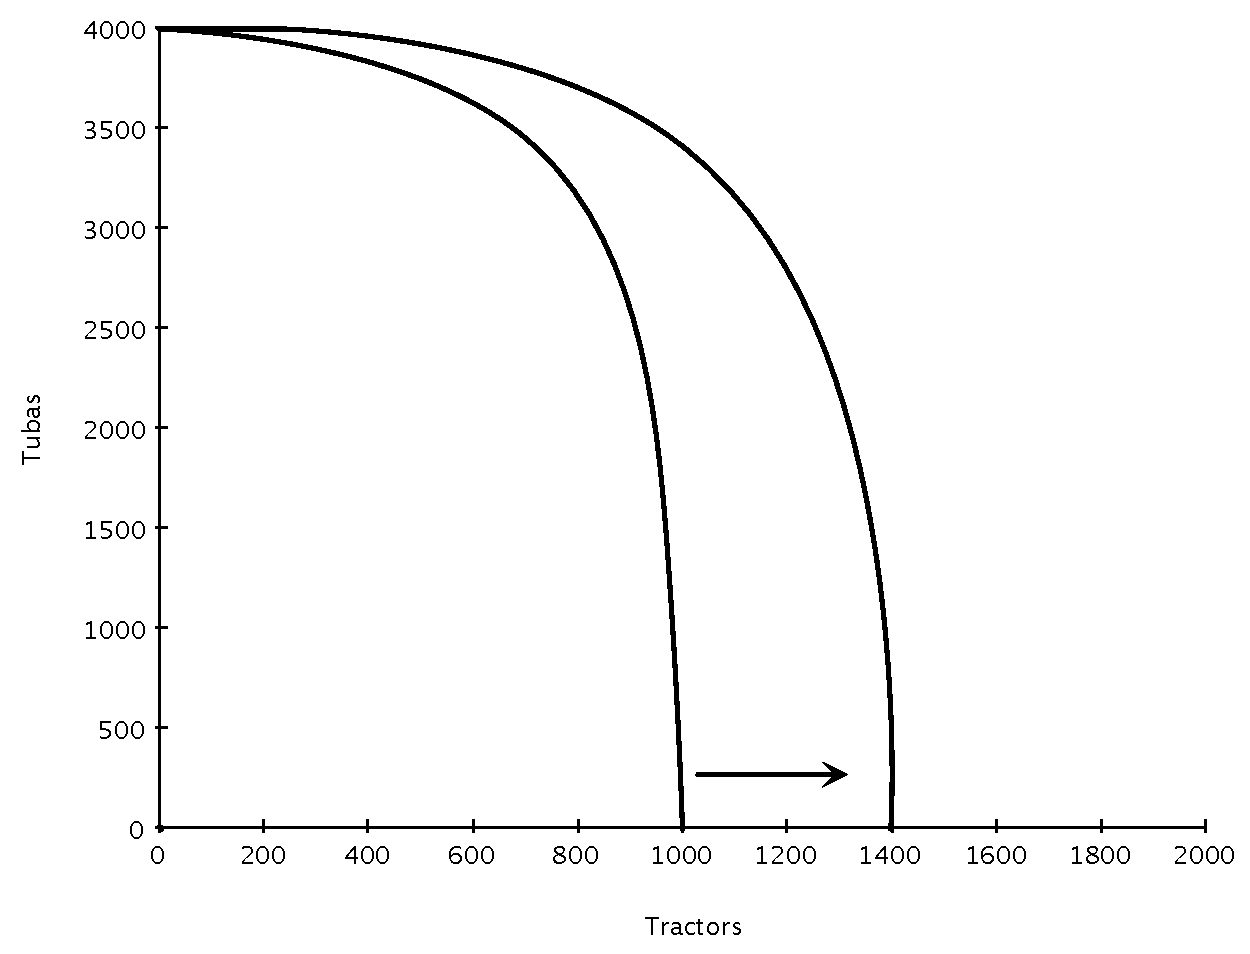
\includegraphics[scale=.2]{plot2.pdf}}
		\caption{Increase in Technology}
		\label{ppf2}
	\end{subfigure}%
	\begin{subfigure}[t]{0.5\textwidth}
		\ddp{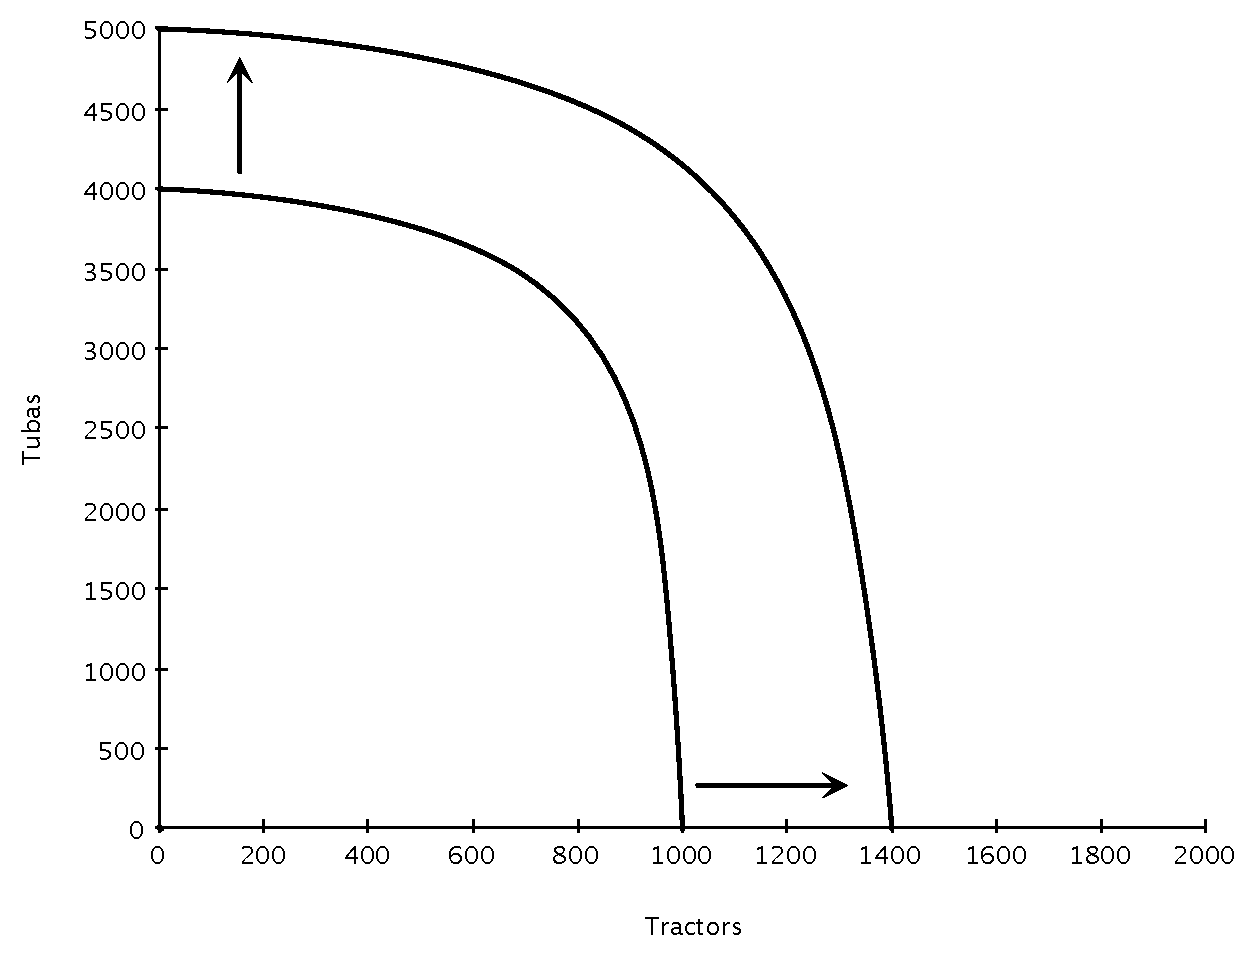
\includegraphics[scale=.2]{plot3.pdf}}
		\caption{Increase in the Labor Force}
		\label{ppf3}
	\end{subfigure}
\end{figure}

\end{frame}

\begin{frame}{The Production Possibilities Frontier}
	\begin{exmp}
		\footnotesize
		A country can produce either guns or butter and their production possibilities frontier is bowed out. If they move from a point where they are producing 25 guns and 30 pounds of butter to one where they are producing 35 guns and 30 pounds of butter, how many of the following statements could account for this?
		
		\begin{enumerate}[i.]
			\item The country saw an influx of workers who specialize in making butter and moved from an efficient point on their former PPF to an efficient point on their new PPF.
			\item A technological breakthrough in gun production allowed the country to move from an efficient point on their former PPF to an efficient point on their new PPF. 
			\item The country moved from an efficient point on their PPF to another efficient point on the same PPF.
			\item The country moved from an inefficient point within their PPF to an efficient point on their PPF.
		\end{enumerate}
	\end{exmp}
\blank
\blank
	\ddp{\pause \small 3 (i, ii, or iv).}
\end{frame}

\begin{frame}{The Production Possibilities Frontier}
	\begin{itemize}
		\item What would the PPF look like if the resources in the economy are not specialized?
		\begin{itemize}
			\item Opportunity costs would \dd{be constant} along entire PPF.
			\item The (absolute) slope of the PPF gives the opportunity cost of the good on the \dd{x-axis}
			\item The reciprocal of the slope gives the opportunity cost of the good on the \dd{y-axis}.
	\end{itemize}
\blank\blank\blank\blank
	\begin{figure}[H]
		\centering
		\ddp{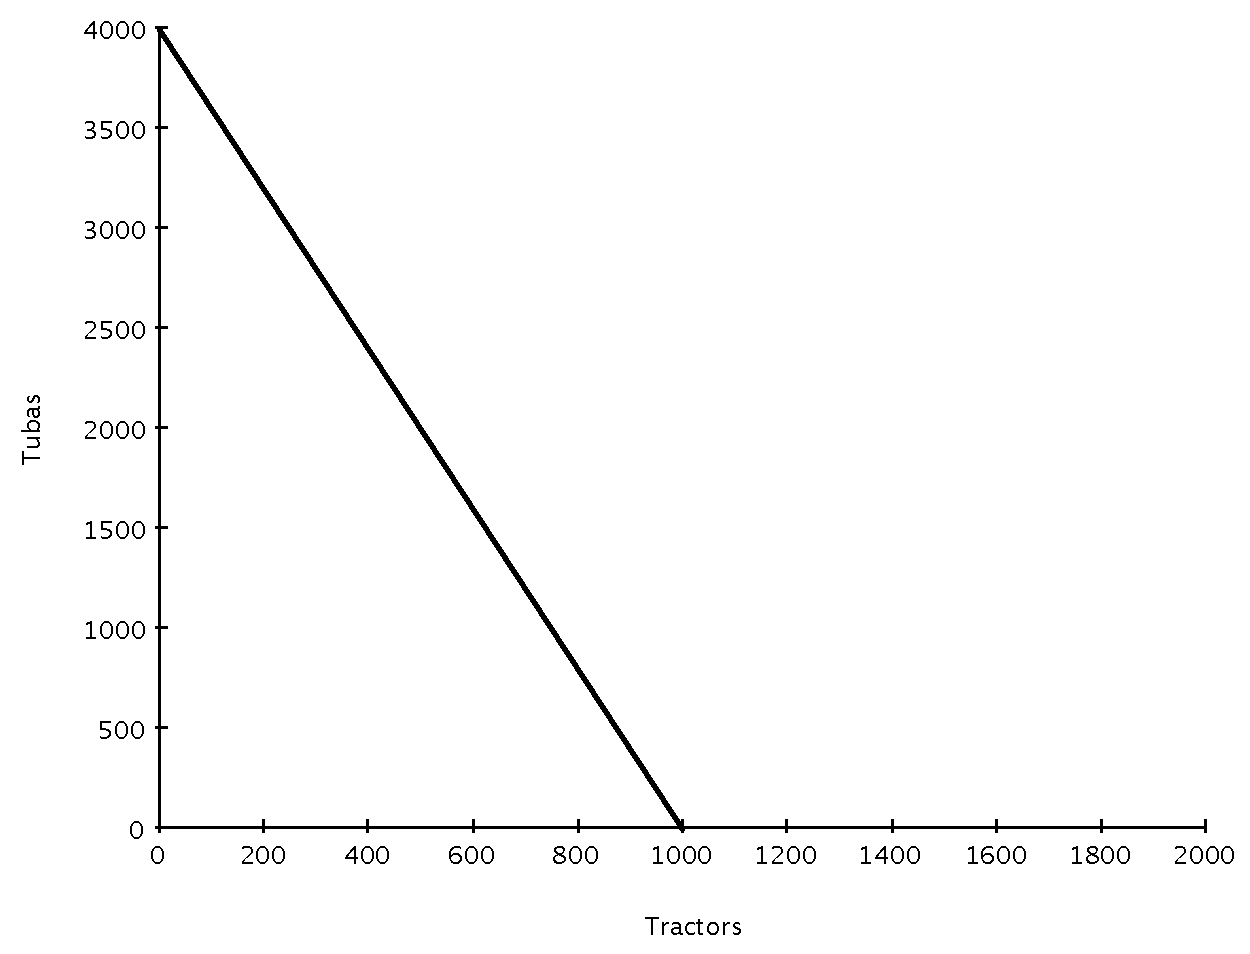
\includegraphics[scale=.2]{plot4.pdf}}
		\caption{Straight-Line PPF}
		\label{ppf4}
	\end{figure}
	\end{itemize}
\end{frame}

\begin{frame}{Readings and Assignments}
\begin{itemize}
		\item Today: Mankiw Ch. 1-2 (skip circular flow diagram)
		\item Next time: Mankiw Ch. 3
		\item Problem Set 1, section 1
\end{itemize}

\end{frame}
	
\end{document}